\section{Why Standard Remedies Fail}
\label{sec:remedies}

The results of \S\ref{sec:results}--\ref{sec:f6} establish CIVO as a failure mode triggered by trained temporal embeddings with multi-rate exposure. We now ask: can standard RL remedies eliminate it? We evaluate seven interventions across four levels (45 intervention experiments across 213 total training runs; Table~\ref{tab:intervention_hierarchy}, Figure~\ref{fig:intervention_heatmap}); none reliably succeeds across environments. The underlying obstacle is structural: in closed-loop imagination, the signal that should correct value bias is itself produced by the model whose estimates require correction.

\begin{figure}[t]
\centering
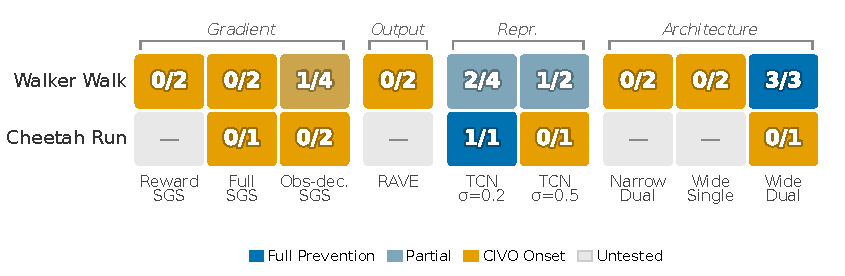
\includegraphics[width=\columnwidth]{figures/paper/fig_intervention_heatmap.pdf}
\caption{Intervention outcomes across environments. Blue = full prevention, light blue = partial, orange = CIVO onset, gray = untested. Only Wide Dual on Walker achieves full prevention (3/3); all other cells show failure or partial results. See Table~\ref{tab:intervention_hierarchy} for complete data.}
\label{fig:intervention_heatmap}
\end{figure}

\begin{table}[t]
\centering
\caption{Intervention hierarchy. Prevention = peak NVE $< 2.0\times$ (35K+). Eval (\%BL) = mean${\pm}$std of final eval return as percentage of per-environment baseline (Walker 915.7, Cheetah 446.1). No level reliably eliminates CIVO across environments.
$^\dagger$Walker 2/4; Cheetah 1/1, PickCube 0/1.
$^\ddagger$Borderline (NVE${=}1.02\times$, eval 55\%).
$^\S$Policy erosion (final 15\% baseline).
$^\|$Walker 3/3, Cheetah 0/1.
$^\#$7 seeds, all NVE $< 2.0\times$.
$^\P$6 seeds, all NVE $< 2.0\times$.}
\label{tab:intervention_hierarchy}
\footnotesize
\setlength{\tabcolsep}{3pt}
\begin{tabular}{llcccc}
\toprule
\textbf{Level} & \textbf{Intervention} & \textbf{Seeds} & \textbf{Prev.} & \textbf{Rate} & \textbf{Eval (\%BL)} \\
\midrule
--- & Untreated & 10 & 0/10 & 0\% & $15{\pm}10$ \\
\midrule
Gradient & Reward-only SGS & 2 & 0/2 & 0\% & $31{\pm}39$ \\
Gradient & Full-pathway SGS & 3 & 0/3 & 0\% & $34{\pm}26$ \\
Gradient & Obs-decoder SGS & 6 & 1/6 & 17\% & $33{\pm}31$ \\
\midrule
Output & RAVE ($c{=}1.5{,}2.0$) & 2 & 0/2 & 0\% & $6{\pm}4$ \\
\midrule
Repr. & TCN ($\sigma{=}0.1$) & 1 & 1/1$^\ddagger$ & 100\% & 21 \\
Repr. & TCN ($\sigma{=}0.2$) & 6$^\dagger$ & 3/6 & 50\% & $14{\pm}7$ \\
Repr. & TCN ($\sigma{=}0.5$) & 3 & 1/3 & 33\% & $20{\pm}11$ \\
Repr. & TCN ($\sigma{=}1.0$) & 1 & 1/1$^\S$ & 100\% & 16 \\
\midrule
Arch. & Wide single & 2 & 0/2 & 0\% & $39{\pm}8$ \\
Arch. & Narrow dual (min) & 2 & 0/2 & 0\% & $70{\pm}8$ \\
Arch. & Wide dual (min) & 4 & 3/4$^\|$ & 75\% & $55{\pm}24$ \\
\midrule
--- & Embedding frozen & 7 & 7/7$^\#$ & 100\% & $31{\pm}18$ \\
--- & Embedding removed & 6 & 6/6$^\P$ & 100\% & $29{\pm}13$ \\
\bottomrule
\end{tabular}
\end{table}

\paragraph{Gradient-level: magnitude does not predict causality.}
Full-SGS (exp\_018) detaches all non-KL gradients from $e_{\dt}$. Seed~1 shows partial mitigation (eval 448.3, NVE $1.66\times$) with late instability (NVE rising from $1.23\times$ mean to $1.66\times$ at 95K), suggesting SGS delays rather than prevents onset; seed~2 collapses entirely (peak ${\sim}488$ at 75K $\to$ 40.8 at 105K), indicating a metastable regime where stochastic factors determine whether delayed onset crosses the critical threshold (Appendix~\ref{sec:sgs_gradient_analysis}). Cross-environment validation on Cheetah confirms CIVO generalization (010b, NVE $8.27$--$108.52\times$); full-SGS yields 0/3 elimination. Removing the embedding eliminates CIVO on Cheetah (024b, NVE $< 0.2\times$). Targeted obs-decoder-only SGS (exp\_025/026) achieves 1/6 prevention (1/4 Walker, 0/2 Cheetah). Reward-only detachment (exp\_016e) produces NVE $10.42\times$---exceeding the untreated maximum ($4.72\times$; Table~\ref{tab:three_way_emb})---by amplifying the obs-decoder pathway (Appendix~\ref{sec:seed_divergence}). The pattern is consistent: blocking any single gradient channel shifts co-adaptation to the remaining ones, and the dominant gradient pathway (observation decoder) is causally inert while the weakest (KL) drives CIVO. Across all gradient variants ($n{=}11$, Table~\ref{tab:intervention_hierarchy}), only 1/11 seeds achieves prevention, confirming pathway redundancy as a structural rather than dosage-dependent limitation.

\paragraph{Output and representation levels: anchors drift and noise shows phase transitions.}
\textbf{RAVE} (value-level capping, $c \in \{1.5, 2.0\}$) fails because the EMA anchor tracks biased values during CIVO onset, rendering the clipping threshold permissive precisely when correction is needed (0/2 prevention, eval $6{\pm}4$\% of baseline---worse than untreated runs, indicating anchor co-drift actively amplifies degradation). \textbf{TCN} (representation-level noise, $\sigma \in \{0.1, 0.2, 0.5, 1.0\}$) shows binary on/off behavior: at $\sigma{=}0.2$, CIVO is suppressed in 2/4 Walker seeds while the remaining seeds escalate to full collapse with no intermediate outcome. No noise level achieves both prevention and performance recovery: mean eval across all TCN configurations ($14$--$21$\% of baseline; Table~\ref{tab:intervention_hierarchy}) remains comparable to untreated runs ($15$\%). The effective dose differs $5\times$ across environments ($\sigma{=}0.2$ partially effective on Walker; $\sigma{=}1.0$ erodes Cheetah policy to 15\% of baseline without preventing CIVO; Appendix~\ref{sec:tcn_cross_env}). This binary dose-response, combined with the absence of a smooth suppression curve, suggests a phase transition between co-adaptation regimes rather than a regularization effect amenable to hyperparameter tuning. We use the term loosely to describe the absence of a smooth dose-response curve; formal characterization of the transition dynamics is left for future work.

\paragraph{Architecture-level: pessimism vanishes in shared-data regimes.}
Dual critics converge across all tested configurations ($n{=}7$): correlation $\rho > 0.999$ with pessimism at only 3--4\% of the independent-critic bound, rendering standard pessimistic value estimation ineffective in pure imagination. The mechanism is structural: both critics train on the same imagined rollouts generated by the same world model, producing identical state-action distributions that drive convergence regardless of random initialization. A $2{\times}2$ factorial separates two components: narrow dual-critic (min, ${\sim}1.2$M) recovers from CIVO after onset (${\sim}16$--$19\times$ NVE ratio reduction) but does not prevent it; wide dual-critic (min $+$ ${\sim}2.4$M) achieves NVE $\leq 1.4\times$ in 3/4 seeds (3/3 Walker, 0/1 Cheetah), the sole positive result across all levels. Wide single (0/2) confirms both min-aggregation and increased capacity are necessary. Cross-environment transfer is limited: the single Cheetah seed (CIVO at $70\times$) exceeds the intervention's capacity, suggesting a severity ceiling (Appendix~\ref{sec:dual_critic_appendix}).

\paragraph{Unifying pattern: closed-loop imagination defeats single-pathway remedies.}
\label{sec:unifying}
The learned model generates both the training distribution and the bootstrap targets for critic updates; any remedy that assumes diverse or independent training sources (Double Q pessimism, EMA anchoring, noise injection) loses its corrective power when both sides of the training signal originate from the same model. Gradient interventions fail from pathway redundancy (blocking one channel amplifies another); output interventions fail from anchor co-drift (the anchor is corrupted by the same bias it should correct); representation interventions exhibit phase transitions (the embedding either co-adapts or does not, with no smooth intermediate); and pessimistic estimation fails from critic convergence (shared rollouts eliminate the diversity that pessimism requires). Only architectural changes that partially break the closed loop (wide dual-critic provides independent capacity that resists convergence) achieve partial prevention, and even this result does not transfer across environments: configurations achieving 3/3 prevention on Walker fail on Cheetah, where CIVO severity is $2$--$20\times$ higher. No single intervention achieves reliable cross-environment prevention: the highest prevention rate (wide dual-critic, 75\%) derives entirely from Walker (3/3 seeds), failing on its sole Cheetah test (0/1).
